\documentclass[tikz,border=4pt]{standalone}
% Shared visual grammar: role fills, dark connectors, and 7-point typography.
% Build each standalone figure from this directory. No external images required.
\pdfinfoomitdate=1
\pdftrailerid{}
\usepackage[T1]{fontenc}
\usepackage{helvet}
\renewcommand{\familydefault}{\sfdefault}
\usepackage{amsmath,amssymb}
\hyphenpenalty=10000
\exhyphenpenalty=10000
\usetikzlibrary{arrows.meta,calc,fit,positioning,decorations.pathreplacing,backgrounds}
\definecolor{ink}{HTML}{172B3A}
\definecolor{muted}{HTML}{586D85}
\definecolor{datafill}{HTML}{F1F5F9}
\definecolor{dataline}{HTML}{62748E}
\definecolor{modelfill}{HTML}{E5E9FF}
\definecolor{modelline}{HTML}{7887C7}
\definecolor{llmfill}{HTML}{FFE4E8}
\definecolor{llmline}{HTML}{E68494}
\definecolor{truthfill}{HTML}{D0FAE5}
\definecolor{truthline}{HTML}{35A782}
\newcommand{\seven}{\fontsize{7}{8.5}\selectfont}
\tikzset{
 every node/.append style={font=\seven,text=ink,align=center},
 box/.style={draw=dataline,fill=white,rounded corners=3pt,line width=.65pt,inner sep=5pt,minimum height=8mm},
 data/.style={box,fill=datafill},
 model/.style={box,draw=modelline,fill=modelfill},
 llm/.style={box,draw=llmline,fill=llmfill},
 truth/.style={box,draw=truthline,fill=truthfill},
 title/.style={font=\seven\bfseries,inner sep=1pt},
 word/.style={text=muted,inner sep=1pt,align=center},
 label/.style={fill=white,inner xsep=2pt,inner ysep=1pt,text=muted},
 flow/.style={-{Stealth[length=2.4mm,width=1.9mm]},draw=ink,line width=1.2pt,shorten >=1.5pt},
 branch/.style={-{Stealth[length=2mm,width=1.6mm]},draw=ink,line width=.9pt,shorten >=1pt},
 route/.style={draw=ink,line width=1.2pt},
 update/.style={-{Stealth[length=2.2mm,width=1.7mm]},draw=modelline,line width=1pt,dash pattern=on 3pt off 2pt,shorten >=1.5pt},
 boundary/.style={draw=dataline,dash pattern=on 3pt off 2pt,rounded corners=3pt,line width=.6pt},
 chip/.style={minimum height=4mm,inner xsep=3pt,inner ysep=1.5pt,rounded corners=2pt},
}
% Optional role key. Anchor at the center of an uncluttered final row.
\newcommand{\rolekey}[2]{
 \node[word,anchor=east] at (#1-6.6,#2) {\textit{Key}};
 \node[data,chip] at (#1-5.2,#2) {records / data};
 \node[model,chip] at (#1-1.9,#2) {learned model / policy};
 \node[llm,chip] at (#1+1.65,#2) {LLM signal};
 \node[truth,chip] at (#1+4.95,#2) {labels / evaluation};
}

\begin{document}
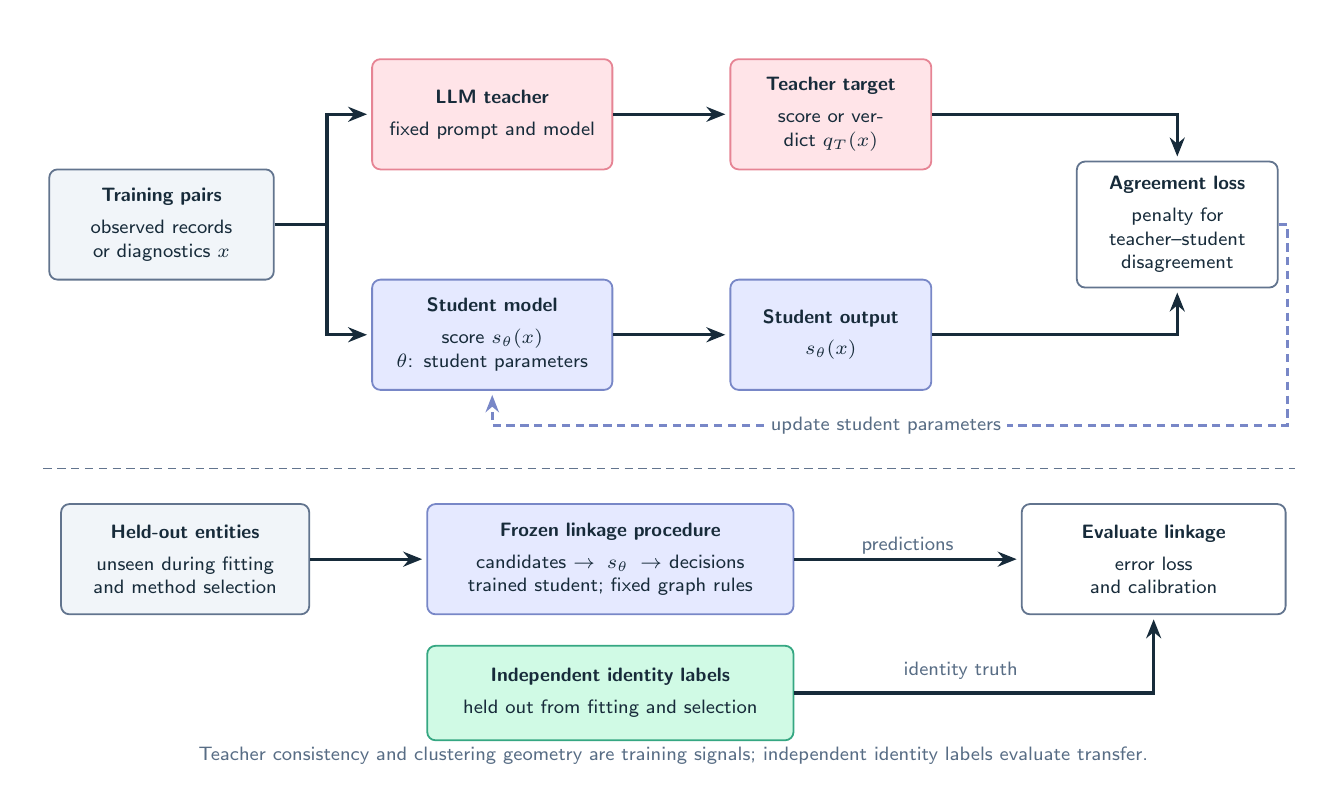
\begin{tikzpicture}

\useasboundingbox (-.2,.3) rectangle (16.1,-9.22);
\node[data,text width=25mm,minimum height=14mm] (x) at (1.5,-2.2) {\textbf{Training pairs}\\[3pt]observed records\\or diagnostics $x$};
\node[llm,text width=27mm,minimum height=14mm] (teacher) at (5.7,-.8) {\textbf{LLM teacher}\\[3pt]fixed prompt and model};
\node[model,text width=27mm,minimum height=14mm] (student) at (5.7,-3.6) {\textbf{Student model}\\[3pt]score $s_\theta(x)$\\$\theta$: student parameters};
\node[llm,text width=22mm,minimum height=14mm] (qt) at (10,-.8) {\textbf{Teacher target}\\[3pt]score or verdict $q_T(x)$};
\node[model,text width=22mm,minimum height=14mm] (qs) at (10,-3.6) {\textbf{Student output}\\[3pt]$s_\theta(x)$};
\node[box,text width=22mm,minimum height=16mm] (loss) at (14.4,-2.2) {\textbf{Agreement loss}\\[3pt]penalty for\\teacher--student\\disagreement};
\draw[route] (x.east) -- (3.6,-2.2);
\draw[flow] (3.6,-2.2) |- (teacher.west); \draw[flow] (3.6,-2.2) |- (student.west);
\draw[flow] (teacher) -- (qt); \draw[flow] (student) -- (qs);
\draw[flow] (qt.east) -- (12,-.8) -| (loss.north);
\draw[flow] (qs.east) -- (12,-3.6) -| (loss.south);
\draw[update] (loss.east) -- (15.8,-2.2) -- (15.8,-4.75) -- (5.7,-4.75) -- (student.south);
\node[label] at (10.7,-4.75) {update student parameters};
\draw[boundary] (0,-5.3) -- (15.9,-5.3);
\node[data,text width=28mm,minimum height=14mm] (held) at (1.8,-6.45) {\textbf{Held-out entities}\\[3pt]unseen during fitting\\and method selection};
\node[model,text width=43mm,minimum height=14mm] (decision) at (7.2,-6.45) {\textbf{Frozen linkage procedure}\\[3pt]candidates $\rightarrow s_\theta\rightarrow$ decisions\\trained student; fixed graph rules};
\node[box,text width=30mm,minimum height=14mm] (evaluate) at (14.1,-6.45) {\textbf{Evaluate linkage}\\[3pt]error loss\\and calibration};
\node[truth,text width=43mm,minimum height=12mm] (truth) at (7.2,-8.15) {\textbf{Independent identity labels}\\[3pt]held out from fitting and selection};
\draw[flow] (held) -- (decision);
\draw[flow] (decision) -- node[label,above] {predictions} (evaluate);
\draw[flow] (truth.east) -- (14.1,-8.15) -- (evaluate.south);
\node[word,anchor=south] at (11.65,-8.02) {identity truth};
\node[word] at (8,-8.95) {Teacher consistency and clustering geometry are training signals; independent identity labels evaluate transfer.};
\end{tikzpicture}
\end{document}
